\documentclass[11pt]{article}
\usepackage[margin=1in]{geometry}
\usepackage{graphicx}
\usepackage{amsmath}
\usepackage{booktabs}
\usepackage{hyperref}
\usepackage{authblk}
\usepackage{enumitem}
\usepackage{setspace}
\usepackage{titlesec}
\usepackage{fancyhdr}

% ---- Clean section headings ----
\titleformat{\section}{\normalfont\Large\bfseries}{\thesection}{1em}{}
\titleformat{\subsection}{\normalfont\large\bfseries}{\thesubsection}{1em}{}

% ---- Header / footer ----
\pagestyle{fancy}
\fancyhf{}
\fancyhead[L]{Deep Hedging vs.\ Black--Scholes Delta Hedging}
\fancyhead[R]{Aryan Gupta}
\fancyfoot[C]{\thepage}
\renewcommand{\headrulewidth}{0.4pt}

\setstretch{1.12}
\setlength{\parskip}{0.5em}

\title{\textbf{Deep Hedging vs.\ Black--Scholes Delta Hedging} \\[4pt]
\large A Personal Quant Finance Implementation Project}
\author[1]{Aryan Gupta}
\affil[1]{Personal Project}
\date{\today}

\begin{document}

\maketitle
\thispagestyle{fancy}

\begin{abstract}
\noindent
This project report documents a personal implementation project in
quantitative finance: building and comparing two option-hedging
strategies -- classical Black--Scholes delta hedging and a
machine-learning-based ``deep hedging'' policy -- under realistic
transaction costs. The project was built independently in Python
(NumPy/SciPy/Matplotlib only) and is inspired by and benchmarked against
the methodology described in Suresh (2026) \cite{suresh2026} and the
deep hedging framework of Buehler et al.\ (2019) \cite{buehler2019}.
Beyond reproducing the core comparison, this project adds a transaction
cost sensitivity sweep to study how the tradeoff between hedging cost and
risk scales with market friction. Full source code is available on
GitHub (link in Section~\ref{sec:code}).
\end{abstract}

\vspace{0.3cm}

\section{Project Overview}
The goal of this project was to answer a practical quant-finance
question: \emph{can a machine-learned hedging policy out-perform the
classical Black--Scholes delta hedge once real trading frictions
(transaction costs) are taken into account?} This required building,
from scratch:

\begin{itemize}[nosep, leftmargin=1.5em]
    \item a market simulator (Geometric Brownian Motion),
    \item a closed-form Black--Scholes pricing and delta-hedging engine,
    \item a small neural-network hedging policy trained without any deep
    learning framework, and
    \item an evaluation pipeline comparing both strategies on cost and
    risk.
\end{itemize}

This project was inspired by and follows the general methodology of
Suresh (2026) \cite{suresh2026}, which compared these same two approaches
in a simulated market. The implementation, code, and the transaction-cost
sensitivity extension described below are my own independent work.

\section{Methodology}

\subsection{Market Simulation}
Stock price paths $S_t$ were generated with Geometric Brownian Motion,
\[
S_{t+\Delta t} = S_t \exp\left[\left(r - \tfrac{1}{2}\sigma^2\right)\Delta t
+ \sigma \sqrt{\Delta t}\, Z_t\right], \qquad Z_t \sim \mathcal{N}(0,1),
\]
under risk-neutral drift, for pricing and hedging a European call option
with strike $K$, risk-free rate $r$, volatility $\sigma$, and maturity
$T$.

\subsection{Black--Scholes Benchmark}
The Black--Scholes call price and delta were computed in closed form at
every rebalancing step. The hedge portfolio was rebalanced to hold
$\Delta_t$ shares of the underlying at each step, with proportional
transaction costs $c \cdot |\text{trade}| \cdot S_t$ deducted from the
cash account, where $c$ is the transaction cost rate.

\subsection{Deep Hedging Policy}
The learned hedging policy is a small feed-forward neural network (one
hidden layer, four hidden units, $\tanh$ activation, sigmoid output)
mapping the current state (moneyness, time-to-maturity) to a target
hedge position in $[0,1]$. Instead of using PyTorch or TensorFlow, the
network was trained directly with \texttt{scipy.optimize} (L-BFGS-B,
numerical gradients), minimizing mean squared terminal profit-and-loss
(P\&L) across simulated training paths, with transaction costs embedded
directly into the P\&L. This keeps the entire project dependency-light
(NumPy, SciPy, Matplotlib) while preserving the core deep hedging idea:
let the optimizer trade off hedge accuracy against trading cost.

\subsection{Extension: Transaction Cost Sensitivity Sweep}
As an extension beyond the base comparison, the deep hedge was retrained
independently at transaction cost rates $c \in \{0.1\%, 0.5\%, 1\%,
2\%\}$ and compared against Black--Scholes at each level, to see how the
size of the cost advantage and the size of the risk penalty change as
trading frictions increase.

\section{Results}

\subsection{Base Comparison}
Using $S_0 = K = \$100$, $r = 2\%$, $\sigma = 20\%$, $T = 0.25$ years,
20 rebalancing steps, and a 1\% transaction cost rate, 500 test paths
produced the results in Table~\ref{tab:results}.

\begin{table}[htbp]
\centering
\renewcommand{\arraystretch}{1.3}
\begin{tabular}{lrr}
\toprule
\textbf{Metric} & \textbf{Black--Scholes} & \textbf{Deep Hedge} \\
\midrule
Mean cumulative transaction cost & 1.959 & 1.439 \\
Mean final P\&L                  & $-2.016$ & $-1.450$ \\
P\&L standard deviation          & 1.001 & 1.111 \\
\bottomrule
\end{tabular}
\caption{Base comparison at a 1\% transaction cost rate. The deep hedge
cut transaction costs by roughly 26.5\% relative to Black--Scholes, at
the cost of higher P\&L volatility -- the same directional tradeoff
reported by Suresh (2026), though the exact magnitude differs due to
independent network architecture, training method, and simulation seed.}
\label{tab:results}
\end{table}

\begin{figure}[htbp]
\centering
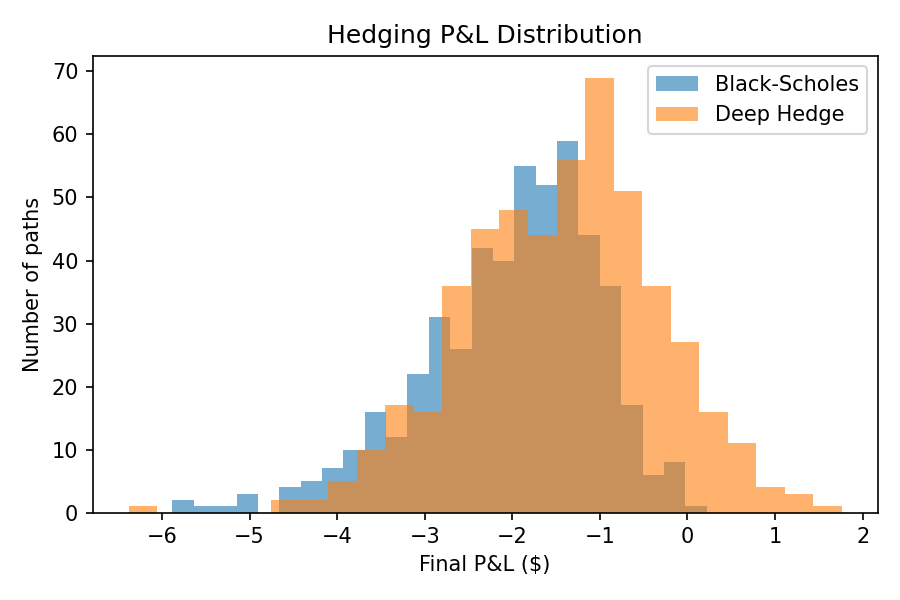
\includegraphics[width=0.65\textwidth]{fig2_pnl_distribution.png}
\caption{Final hedged P\&L distribution across simulated paths. The
Black--Scholes hedge is tighter; the deep hedge accepts more variance
in exchange for lower trading costs.}
\label{fig:pnl}
\end{figure}

\subsection{Cost Sensitivity Sweep}
Figure~\ref{fig:sweep} shows the sweep across transaction cost rates.
The deep hedge's cost advantage grows with the cost rate -- at
$c = 0.1\%$ the two strategies cost about the same, while at $c = 2\%$
the deep hedge costs roughly 46\% less than Black--Scholes. This
indicates the learned policy only meaningfully departs from continuous
delta hedging once frictions make doing so worthwhile.

\begin{figure}[htbp]
\centering
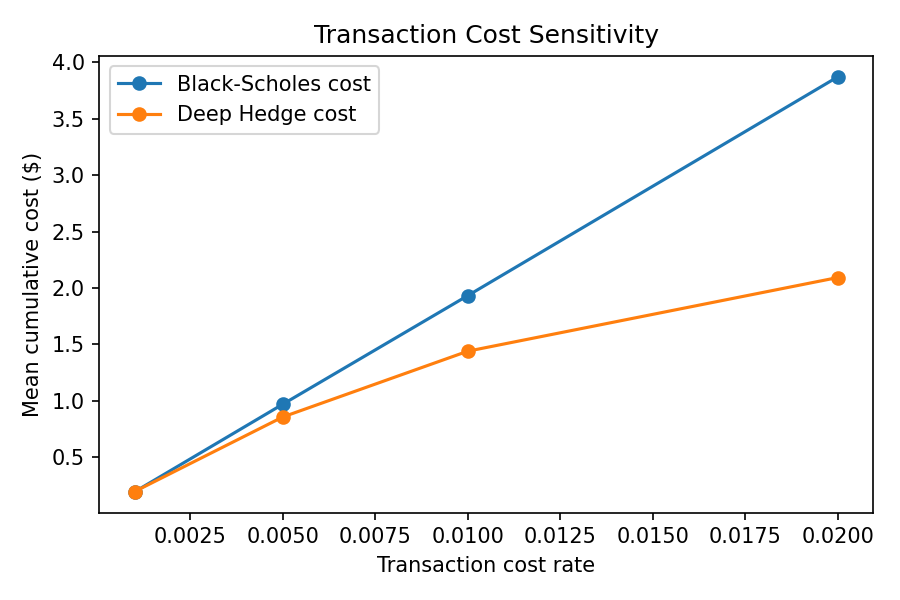
\includegraphics[width=0.65\textwidth]{fig4_cost_sensitivity.png}
\caption{Mean cumulative transaction cost vs.\ transaction cost rate for
both strategies.}
\label{fig:sweep}
\end{figure}

\section{Skills Demonstrated}
\begin{itemize}[nosep, leftmargin=1.5em]
    \item Monte Carlo / stochastic process simulation (GBM)
    \item Closed-form derivatives pricing (Black--Scholes)
    \item Numerical optimization for policy learning (gradient-free
    training of a neural network without a deep learning framework)
    \item Risk/cost tradeoff analysis and sensitivity testing
    \item Data visualization and results reporting
    \item Reproducible, dependency-light scientific Python code
\end{itemize}

\section{Limitations}
The market model is a simplified GBM with constant volatility, no jumps,
and no bid-ask spread beyond the proportional cost term. The network is
intentionally small and trained via numerical optimization rather than
full backpropagation; a larger network trained end-to-end with a deep
learning framework could produce different results. All results are
based on simulated data and have not been validated against historical
markets.

\section{Conclusion}
This project independently implemented and compared Black--Scholes delta
hedging with a machine-learning-based deep hedging policy under
transaction costs, confirming the directional tradeoff described in
Suresh (2026): learned hedging can reduce trading costs at the expense
of higher P\&L volatility. The added transaction-cost sensitivity sweep
shows this advantage grows with the size of market frictions. Natural
next steps include a stochastic volatility model, an explicit
risk-adjusted (e.g., CVaR) training objective, and backtesting on
historical data.

\section{Code Availability}
\label{sec:code}
Full source code, README, and setup instructions are available at:
\url{https://github.com/YOUR-USERNAME/deep-hedging-project}
(update this link once your repository is live).


\begin{thebibliography}{9}

\bibitem{suresh2026}
Suresh, M. (2026). Deep Hedging Under Transaction Costs: A Comparison
with Black--Scholes Delta Hedging. \emph{SSRN Working Paper}.

\bibitem{black1973}
Black, F., and Scholes, M. (1973). The Pricing of Options and Corporate
Liabilities. \emph{Journal of Political Economy}, 81(3):637--654.

\bibitem{buehler2019}
Buehler, H., Gonon, L., Teichmann, J., and Wood, B. (2019). Deep Hedging.
\emph{Quantitative Finance}, 19(8):1271--1291.

\end{thebibliography}

\end{document}